
\begin{figure}[h]
\centering
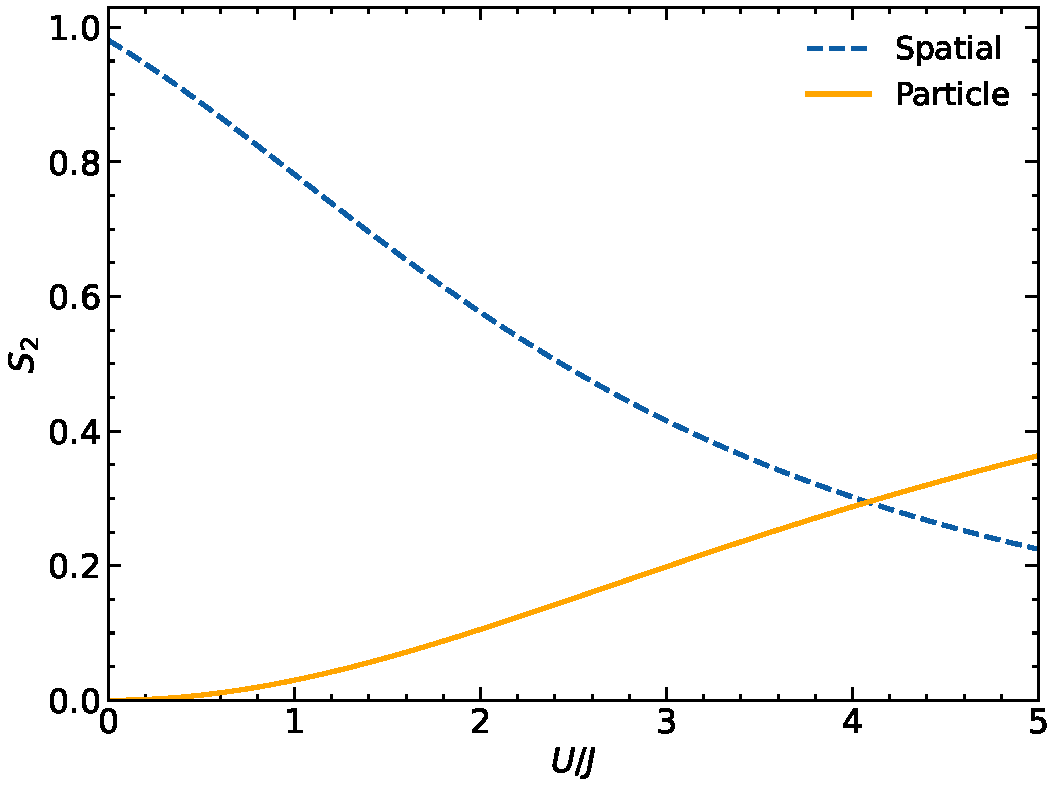
\includegraphics[scale=0.5]{../figures/ed_renyi.pdf}
\caption{The figure above is a graph of the Renyi entanglement entropy for both spatial and particle bipartitions versus the ratio of the interaction term to the hopping term.}
\end{figure}

\subsection{PIGSFLI Algorithm} \label{PIGSFLI}

A Monte Carlo simulation is a stochastic (random) method of integration, which allows for accurate estimations of desired values. Monte Carlo is necessary for situations where exact calculations are too computationally expensive, such as in the exact diagonalization of the reduced density matrix for high particle/site number Bose Hubbard systems. The size of the Hilbert space is calculated by \cref{eq:36} and shown by \cref{fig:hilbert_space_size}:

\begin{equation}
D = \frac{\left(N+L-1\right)!}{\left(N\right)!\left(L-1\right)!}
\label{eq:36}
\end{equation}

\begin{figure}[h]
\centering
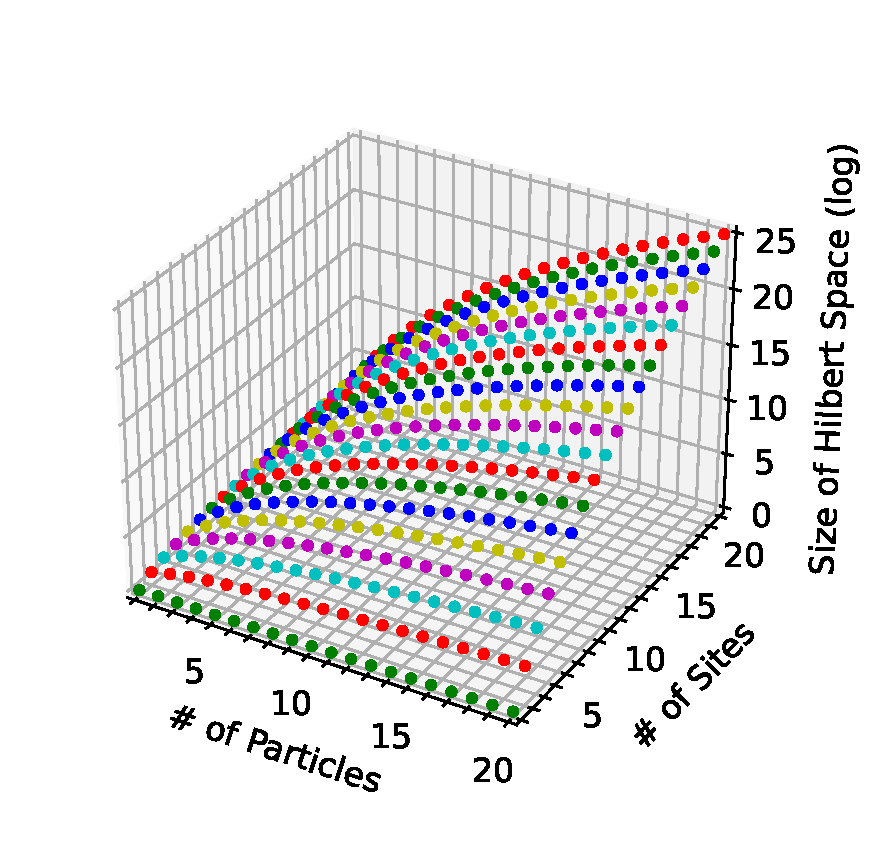
\includegraphics[scale=0.5]{../figures/hilbert_space_size.pdf}
\caption{The figure above shows the size of the Hilbert space as a function of number of sites and particles. This 3-dimensional plot for the number of combinations in the Hilbert space goes up to $20$ sites and $20$ particles.}
\label{fig:hilbert_space_size}
\end{figure}


\begin{figure}[H]
\centering
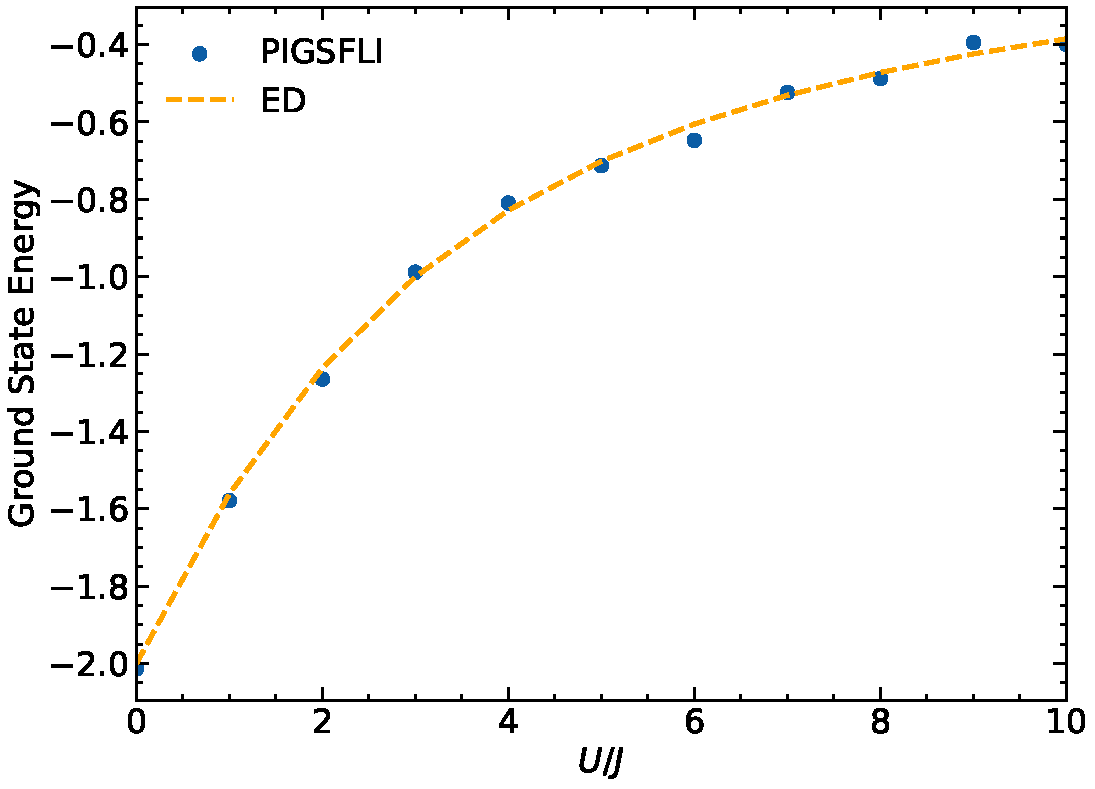
\includegraphics[scale=0.5]{../figures/total_energy.pdf}
\caption{A plot of the ground state energy versus the ratio between U, the potential term, and J, the hopping term for both exact diagonalization and PIGSFLI algorithm. From this plot, the PIGSFLI reults match very well to our ED calculation.}
\label{fig:total_energy}
\end{figure}

\begin{figure}[H]
\centering
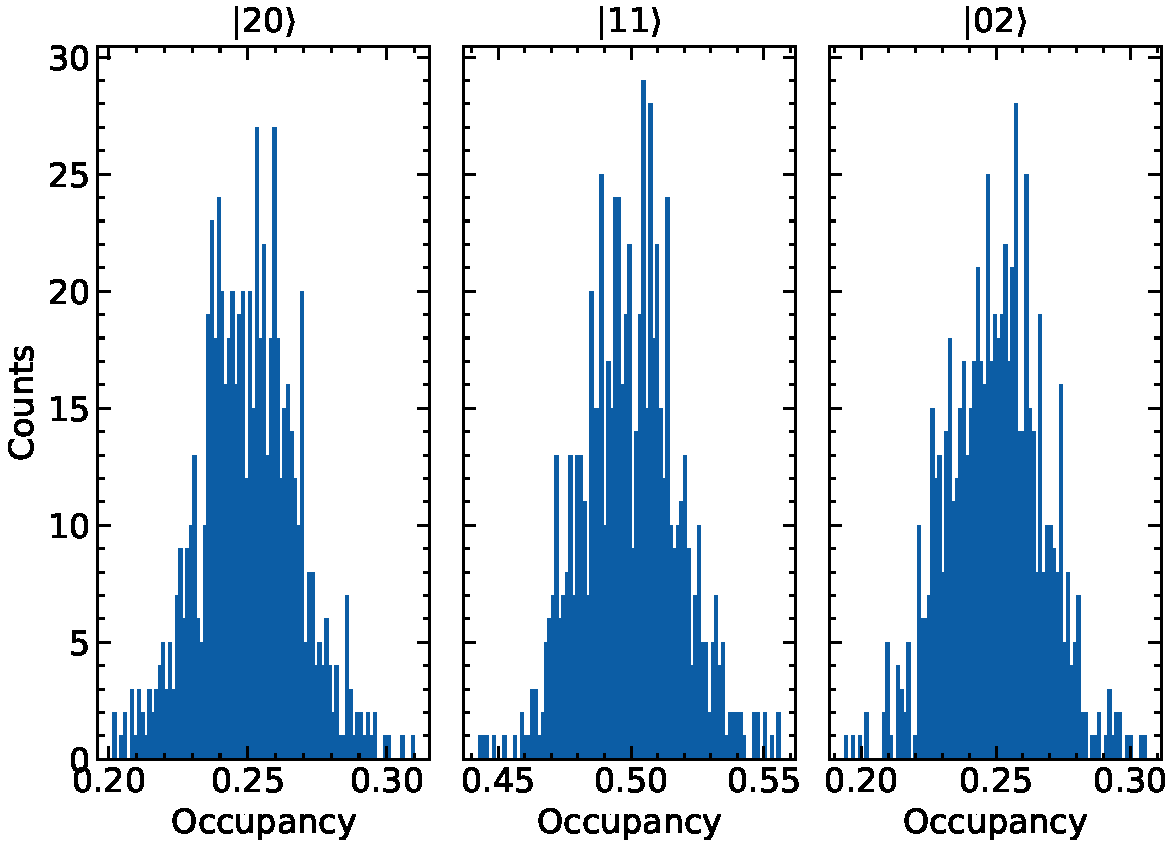
\includegraphics[scale=0.5]{../figures/sep_occ_hist_U_0.0001.pdf}
\caption{The figure above shows the histogram of the occupation number for the particle bipartition as a function of the ratio of the interaction term to the hopping term. This graph specifically shows the case where the interaction term is a tenth of the hopping term.}
\label{fig:sep_occ_hist_U_0.0001}
\end{figure}

\begin{figure}[H]
\centering
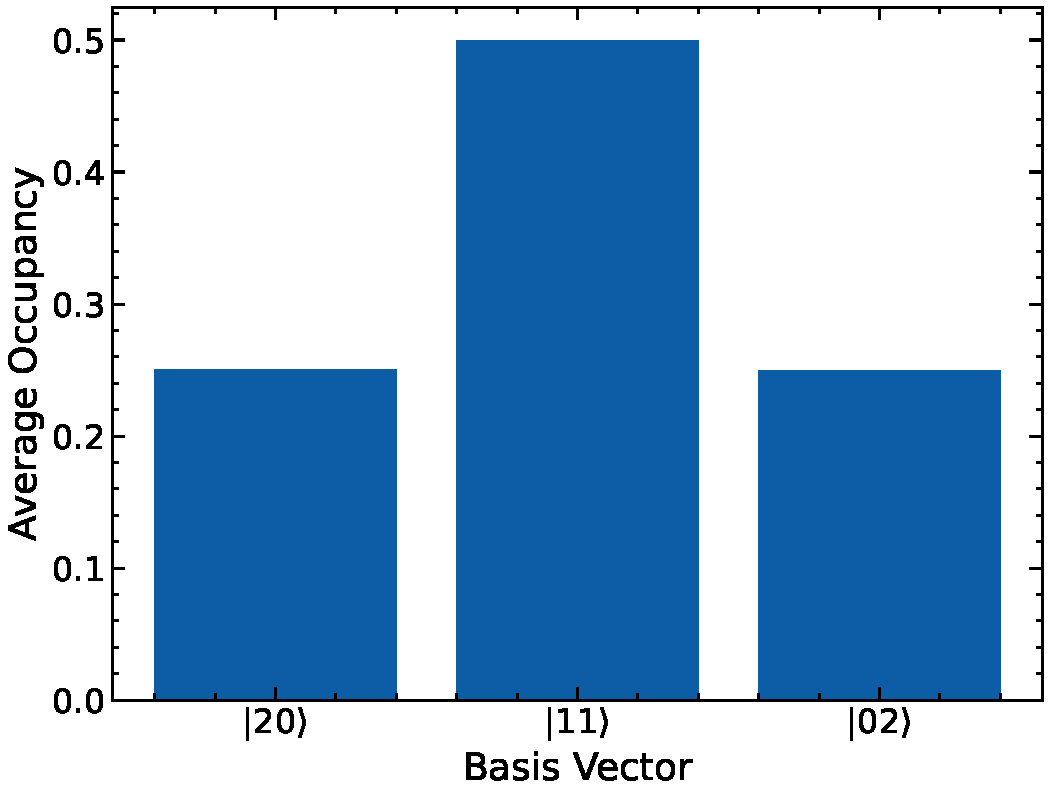
\includegraphics[scale=0.5]{../figures/spatial_avg_occ_U_0.0001.pdf}
\caption{The figure above shows the average occupation number for the spatial bipartition as a function of the ratio of the interaction term to the hopping term. This graph specifically shows the case where the interaction term is a tenth of the hopping term.}
\label{fig:spatial_avg_occ_U_0.0001}
\end{figure}

\begin{figure}[H]
\centering
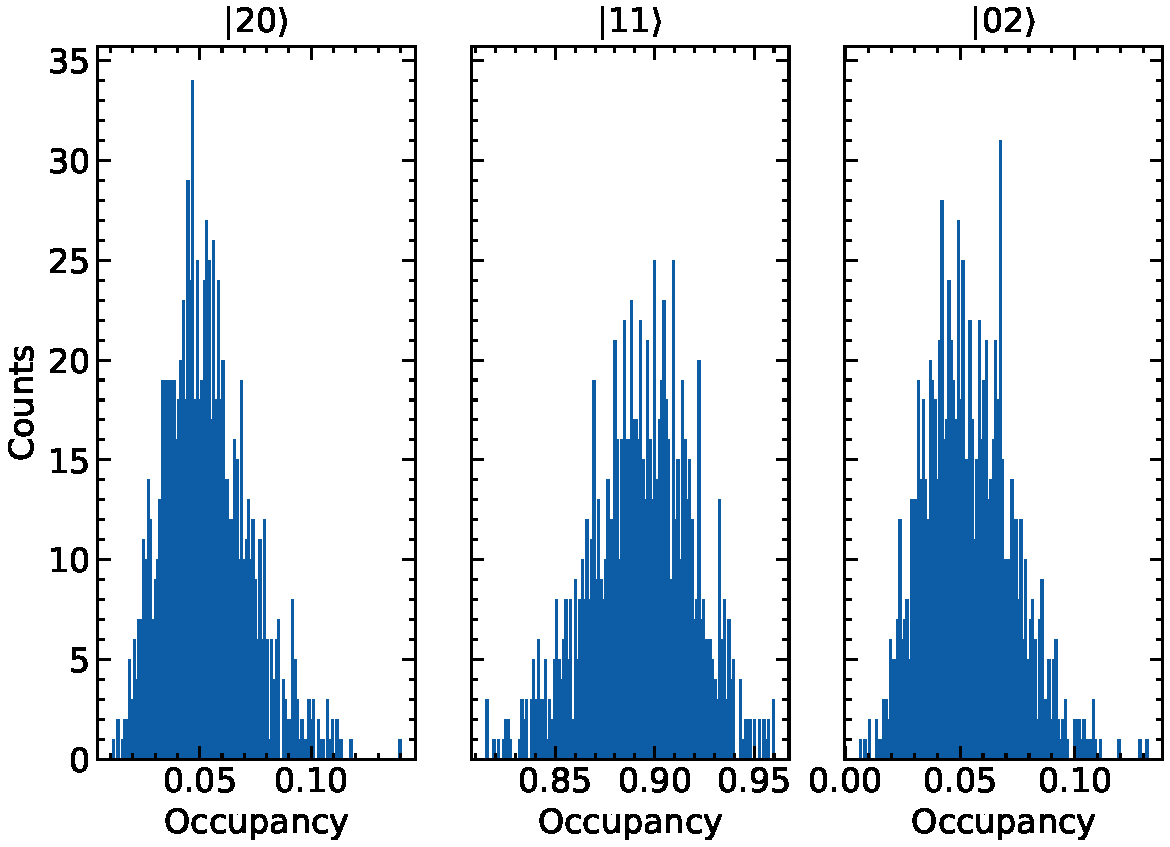
\includegraphics[scale=0.5]{../figures/sep_occ_hist_U_10.0000.pdf}
\caption{The figure above shows the histogram of the occupation number for the spatial bipartition as a function of the ratio of the interaction term to the hopping term. This graph specifically shows the case where the interaction term is $10$ times the hopping term.}
\label{fig:spatial_occ_hist_U_10.0000}
\end{figure}

\begin{figure}[H]
\centering
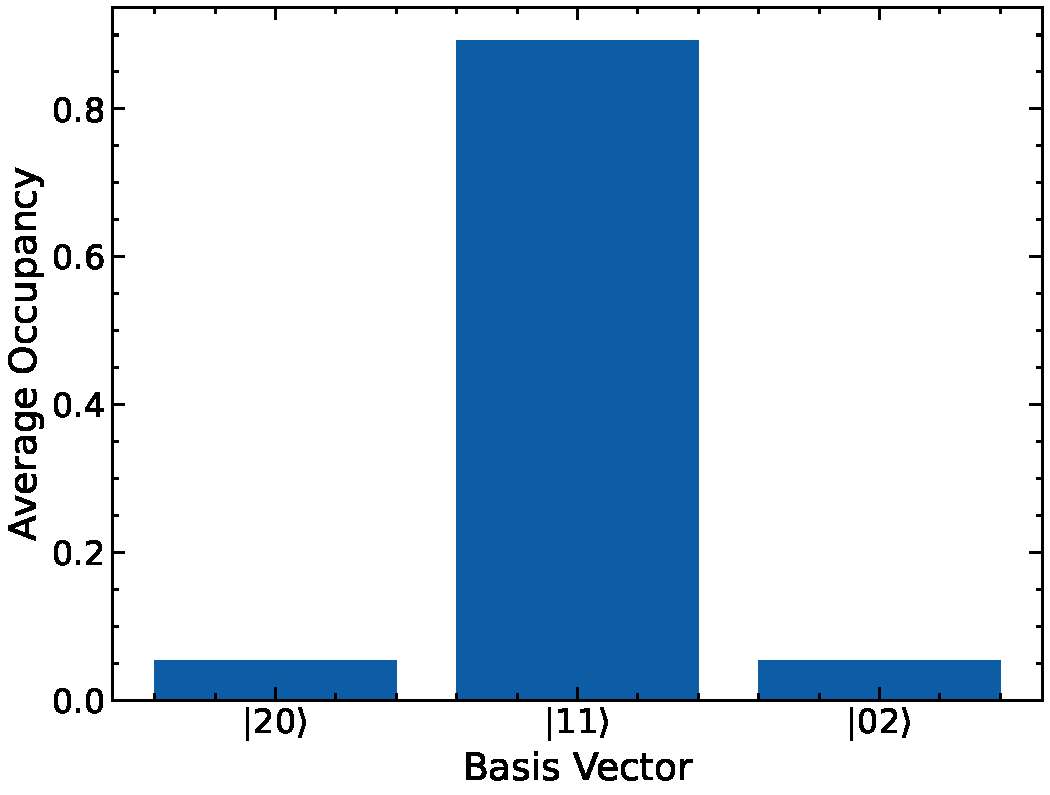
\includegraphics[scale=0.5]{../figures/spatial_avg_occ_U_10.0000.pdf}
\caption{The figure above shows the average occupation number for the spatial bipartition as a function of the ratio of the interaction term to the hopping term. This graph specifically shows the case where the interaction term is $10$ times the hopping term.}
\label{fig:spatial_avg_occ_U_10.0000}    
\end{figure}


\subsubsection{Comparison of PIGSFLI to Exact Diagonalization} \label{results}
\begin{figure}[H]
\centering
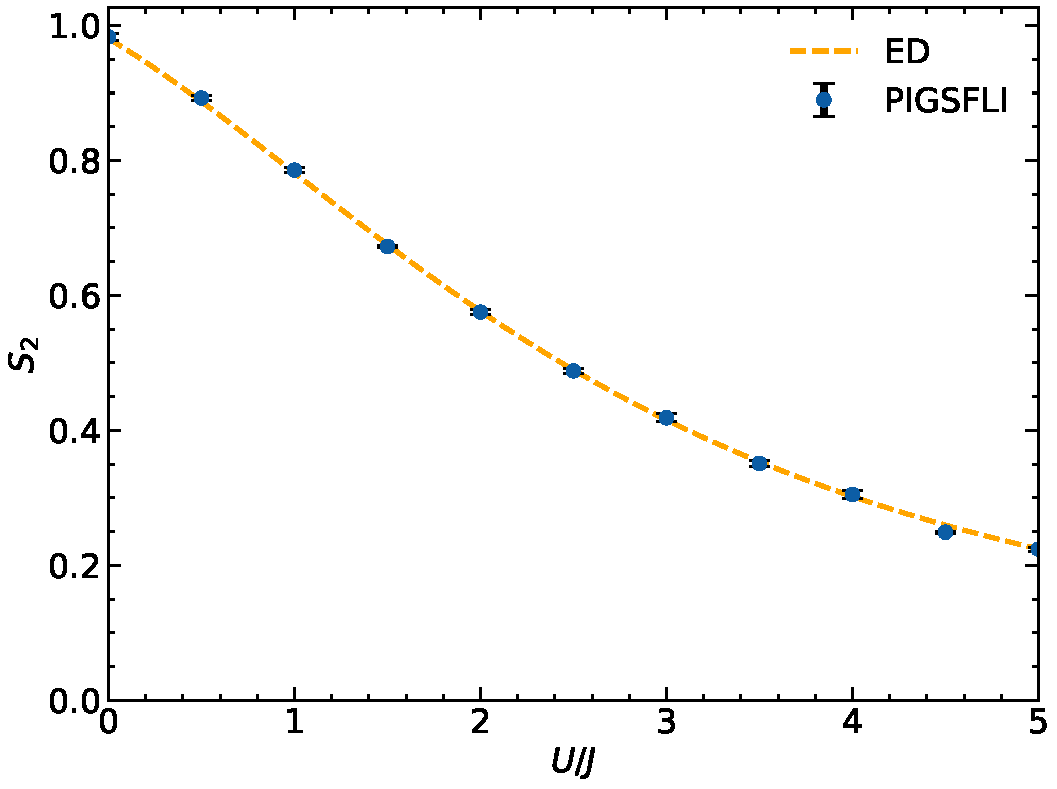
\includegraphics[scale=0.5]{../figures/renyi_spatial.pdf}
\caption{The second Rényi spatial entanglement entropy as a function of U/J for both exact diagonalization (ED) and PIGSFLI. This plot shows excellent agreement between the PIGSFLI estimation and that of our ED calculation, showing that PIGSFLI is a viable option for computation on much larger system sizes.}
\label{fig:renyi_spatial}
\end{figure}

\subsection{Introduction to Machine Learning for Scientists}

While working with the DelMaestro group and attending lectures held during the QAO REU at the University of Tennessee Koxville, I was exposed to machine learning as a tool for physicists and other scientists alike. 

\subsubsection{Applications of DNN to Physics}

\begin{description}
\item [Application:] Learning the Energy Potential
\item [Description:] Train network on small system sizes (which we know the exact solution for), then extrapolate for application of larger system sizes 

\item [Application:] Phase Discrimination
\item [Description:] Supervised and un-supervised 

\item[Application:] Variational Ansatz 
\item[Description:] 

\item [Application:] Solving the Schrodinger Equation
\item[Description:] 

\item [Application:] Speeding up Monte Carlo
\item [Description:] 
\end{description}

\subsubsection{Basic Neural Networks}

\begin{figure}[H]
\centering
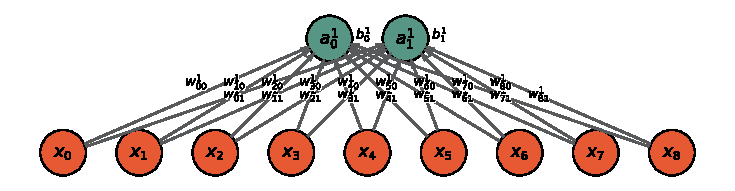
\includegraphics{../figures/neural_network.pdf}
\caption{The figure above is an example of a simple feed-forward neural network, taking in nine inputs and returning two outputs.}
\end{figure}

\noindent \textbf{Neural Network:} non-linear function of many variables that depends on a large number of parameters \\
\textbf{Deep Neural Network:} a neural network with one or more hidden layers (i.e., not an input or output layer)

\begin{figure}[H]
\centering
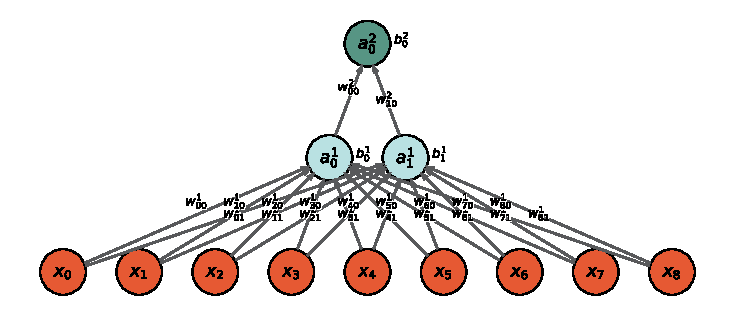
\includegraphics{../figures/DNN.pdf}
\caption{The figure above is an example of a simple feed-forward deep neural network, taking in nine inputs and returning one output with one hidden layer between the input and output layers.}
\end{figure}
			
\subsubsection{Visualizing Feed Forward}

Some examples to visualize complexity generated from simple feed forward neural network with 2 input parameters and 2 hidden layers with 200 nodes each are shown below:

\begin{figure}[H]
\centering
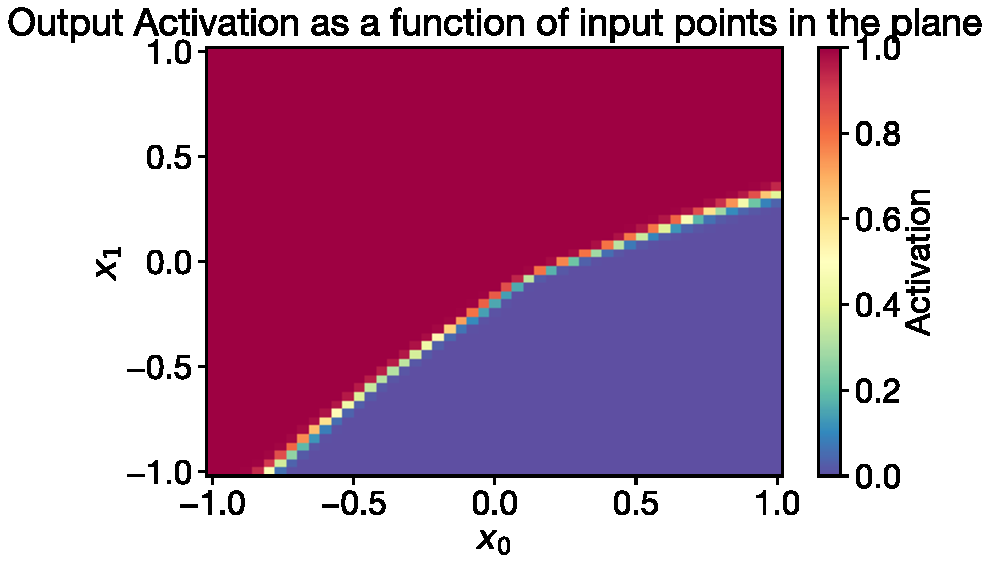
\includegraphics[scale=0.65]{../figures/activation_heat_map.pdf}
\caption{The figure above is the activation output as a function of the two input parameters $x_0$ and $x_1$, which were randomly generated. The activation is calculated through use of the sigmoid function. Specifically, this is a heat map where the color is associated with the activation level.}
\end{figure}

\begin{figure}[H]
\centering
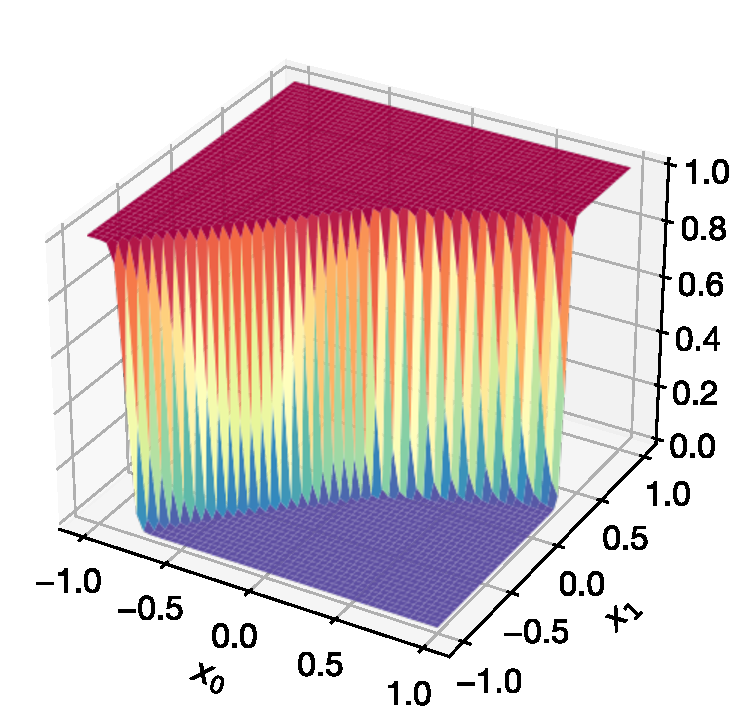
\includegraphics[scale=0.65]{../figures/activation_3d.pdf}
\caption{The figure above is the activation output as a function of the two parameters $x_0$ and $x_1$, which were randomly generated. The activation is calculated through use of the sigmoid function. Specifically, this is a heat map in 3-dimensional space where the activation is the on the vertical axis.}
\end{figure}

\subsubsection{Batch Processing}

\subsubsection{Linear Regression}
\subsubsubsection{Linear Regression Example}
The radioactive decay of an unknown sample is described by the following equation:
\begin{equation}
N(t) = N(0) e^{-t/\tau},
\end{equation}
where $N(t)$ is the number of atoms at time $t$, $N(0)$ is the number of atoms at time $t=0$, $t$ is the time in seconds, and $\tau$ is the time constant of the decay. The above equation can be rearranged into a linear relationship of the form 
\begin{equation}
N(t) = \ln{\left( N(0) \right)} - \frac{1}{\tau}t.
\end{equation}
For our simple feed forward neural network, this is similar to the following form:
\begin{equation}
F = w_o + w_1t,
\end{equation}
were $F$ is the function we're trying to fit, $w_0$ and $w_1$ are the weights, which are (potentially non-linear) functions of the unknown parameters $N(0)$ and $\tau$, and $t$ is the time in seconds. Plotting the original data as well as the linear regression calculation, we find the following:
\begin{figure}[H]
\centering
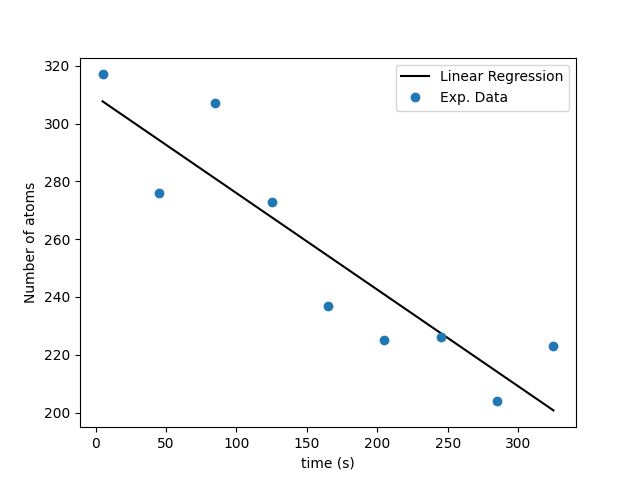
\includegraphics[scale=0.75]{../figures/decay_data.png}
\caption{This figure is a plot of the number of atoms versus time passed in seconds. The blue data points in the figure above represent the experimental data and the black line represents the linear fit to this data using a simple feed-forward neural network.}
\end{figure}

\subsubsection{Feature Maps}

\subsubsection{Model Complexity}